% =============================================================================
%  中文期刊论文 LaTeX 模板（ctexart + XeLaTeX，默认单栏投稿稿）
% -----------------------------------------------------------------------------
%  编译方式（推荐）：
%      latexmk -xelatex PaperTemplate.tex
%  或手动四步：
%      xelatex PaperTemplate.tex
%      bibtex  PaperTemplate
%      xelatex PaperTemplate.tex
%      xelatex PaperTemplate.tex
%
%  字体：
%     默认 fontset=windows（宋体/黑体/楷体/仿宋，Windows 本地编译）
%     Overleaf 或无 Windows 字体的环境改用 fontset=fandol（见下方注释）
%
%  说明：本模板用于中文期刊论文的写作与 PDF 稿排版，最终投稿格式
%        请以目标期刊官方指南为准。
%  图片：支持 PNG / JPG / PDF，也支持 EPS（需 Ghostscript，TeX Live 自带）。
% =============================================================================

% ------------------------------- 文档类 --------------------------------------
% 默认：单栏投稿稿（A4，正文小四，1.5 倍行距）
\documentclass[UTF8, a4paper, zihao=-4, fontset=windows]{ctexart}
% 无 Windows 字体（Overleaf、Linux 服务器）时，注释上一行、改用：
% \documentclass[UTF8, a4paper, zihao=-4, fontset=fandol]{ctexart}
% 本文件为单栏投稿稿；双栏定稿版见同目录 PaperTemplate-twocol.tex
% （首页通栏、正文两栏，编译方式：latexmk -xelatex PaperTemplate-twocol.tex）。

% ------------------------------- 页面设置 ------------------------------------
\usepackage[a4paper, top=2.5cm, bottom=2.5cm, left=2.8cm, right=2.8cm,
            headheight=15pt, headsep=0.5cm, footskip=1.0cm]{geometry}

% ------------------------------- 数学宏包 ------------------------------------
\usepackage{amsmath}        % align、equation、aligned 等公式环境
\usepackage{amssymb}        % 额外数学符号
\usepackage{bm}             % 粗体数学符号 \bm

% ------------------------------- 图形表格 ------------------------------------
\usepackage{graphicx}       % 插图
% EPS 图片支持：
%   XeLaTeX 下由 xetex.def 调用 Ghostscript 直接把 EPS 转成 PDF 图形；
%   pdfLaTeX 下由 epstopdf 在编译时自动转换（同样需要 Ghostscript 在 PATH 中，
%   TeX Live 会优先使用自带的 Ghostscript）。
\usepackage{iftex}
\ifPDFTeX
  \usepackage{epstopdf}
\fi
\usepackage{subcaption}     % 子图 (a)(b)（同时加载 caption）
\usepackage{xcolor}         % 颜色（须在 diagbox/tikz 之前加载）
\usepackage{multirow}       % 表格多行合并
\usepackage{booktabs}       % 三线表 \toprule/\midrule/\bottomrule
\usepackage{diagbox}        % 表头斜线单元格（依赖 tikz）

% ------------------------------- 算法 ----------------------------------------
\usepackage{algorithm}      % 算法浮动体
\usepackage{algpseudocode}  % 伪代码

% ------------------------------- 定理与版式 ----------------------------------
\usepackage{amsthm}         % 定理环境
\usepackage{mdframed}       % 带边框的文本框
\usepackage{comment}        % 大段注释
\usepackage{url}            % URL 自动换行
\usepackage{fancyhdr}       % 页眉页脚
\usepackage{etoolbox}       % 环境钩子（用于设置参考文献字号）

% ------------------------------- 参考文献 ------------------------------------
% 注意：gbt7714 会自行加载 natbib（GB/T 7714 顺序编码制所需的引用机制），
%       因此不再加载 cite / citesort（详见 README 与文末注释）。
\usepackage[unicode, hidelinks, bookmarksnumbered=true, bookmarksopen=true,
            hyperfootnotes=false]{hyperref}
\usepackage{gbt7714}

% =============================== 自定义 ======================================

% 页面 1.5 倍行距、首行缩进 2 字符
\linespread{1.5}\selectfont
\setlength{\parindent}{2em}
\setlength{\parskip}{0pt}

% 页脚居中页码
\pagestyle{fancy}
\fancyhf{}
\fancyfoot[C]{\zihao{5}\thepage}
\renewcommand{\headrulewidth}{0pt}
\renewcommand{\footrulewidth}{0pt}

% 标题与作者信息：直接在下方“中文标题信息”处填写（黑体三号居中）

% 章节标题：
%   一级标题 黑体四号；二级标题 黑体小四；三级标题 黑体五号
\ctexset{
  section = {
    format     = {\heiti\zihao{4}\raggedright},
    name       = {,},
    aftername  = \hspace{0.5em},
    beforeskip = {1.2ex plus 0.2ex minus 0.2ex},
    afterskip  = {0.8ex plus 0.2ex},
  },
  subsection = {
    format     = {\heiti\zihao{-4}\raggedright},
    name       = {,},
    aftername  = \hspace{0.5em},
    beforeskip = {0.9ex plus 0.2ex},
    afterskip  = {0.6ex plus 0.2ex},
  },
  subsubsection = {
    format     = {\heiti\zihao{5}\raggedright},
    name       = {,},
    aftername  = \hspace{0.5em},
    beforeskip = {0.6ex plus 0.2ex},
    afterskip  = {0.4ex plus 0.2ex},
  },
}

% 图表标题：五号黑体；图题在下、表题在上
\DeclareCaptionFont{capfont}{\heiti\zihao{5}}
\DeclareCaptionFont{subcapfont}{\songti\zihao{-5}}
\captionsetup{font=capfont, labelsep=quad, skip=4pt}
\captionsetup[figure]{position=bottom}
\captionsetup[table]{position=top}
\captionsetup[sub]{font=subcapfont, labelsep=space}

% 浮动体与正文间距
\setlength{\textfloatsep}{10pt plus 2pt minus 2pt}
\setlength{\floatsep}{8pt plus 2pt minus 2pt}
\setlength{\intextsep}{8pt plus 2pt minus 2pt}

% 中文图表名、参考文献名（ctex 默认已是“图/表/参考文献”，此处显式声明便于修改）
\renewcommand{\figurename}{图}
\renewcommand{\tablename}{表}
\renewcommand{\refname}{参考文献}

% 修订标记：删除标红、新增标蓝（与 IEEE 模板中的同名宏一致）
\newcommand{\textdelet}[1]{\textcolor{red}{#1}}   % \textdelet{被删除的文字}
\newcommand{\textadd}[1]{\textcolor{blue}{#1}}    % \textadd{新增的文字}

% 中文定理环境（amsthm）
\theoremstyle{plain}
\newtheorem{theorem}{定理}
\newtheorem{lemma}{引理}
\newtheorem{corollary}{推论}
\theoremstyle{definition}
\newtheorem{remark}{注}
\theoremstyle{plain}
\newtheorem{proposition}{命题}
\renewcommand{\proofname}{证明}

% 算法环境：中文标题与中文输入/输出标签
\floatname{algorithm}{算法}
% 算法标题同样设为五号黑体，与图题、表题保持一致
% （注意：float 宏包 ruled 风格会给标题标签加粗，这里显式指定 labelfont，
%   避免出现 SimHei 粗体字形缺失的字体警告。）
\captionsetup[algorithm]{font=capfont, labelfont=capfont, labelsep=quad, skip=4pt}
\algrenewcommand\algorithmicrequire{\textbf{输入：}}
\algrenewcommand\algorithmicensure{\textbf{输出：}}
% 如需把伪代码关键字全部改为中文，取消下面注释即可：
% \algrenewcommand\algorithmicwhile{\textbf{当}}
% \algrenewcommand\algorithmicdo{\textbf{执行}}
% \algrenewcommand\algorithmicend{\textbf{结束}}
% \algrenewcommand\algorithmicfor{\textbf{对}}
% \algrenewcommand\algorithmicif{\textbf{如果}}
% \algrenewcommand\algorithmicthen{\textbf{则}}
% \algrenewcommand\algorithmicelse{\textbf{否则}}
% \algrenewcommand\algorithmicreturn{\textbf{返回}}

% 首行无标记脚注（用于基金项目、作者简介）
% 说明：\thefootnote 置空以隐藏标记；同时给出唯一的 \theHfootnote，
%       避免 hyperref 报 “Ignoring empty anchor” 警告。
\newcounter{blfootnote}
\newcommand{\blfootnote}[1]{%
  \begingroup
  \stepcounter{blfootnote}%
  \renewcommand{\thefootnote}{}%
  \renewcommand{\theHfootnote}{blfootnote.\arabic{blfootnote}}%
  \footnotetext{#1}%
  \endgroup
}

% hyperref 元信息（PDF 属性，可按需修改）
\hypersetup{
  pdftitle  = {面向6G的近场非正交多址接入系统资源分配方法},
  pdfauthor = {张三，李四，王五},
  pdfkeywords = {非正交多址接入；近场通信；波束成形；资源分配},
}

% 参考文献正文：宋体小五（gbt7714 已加载 natbib，此处仅调整字号字体）
\AtBeginEnvironment{thebibliography}{\zihao{-5}\songti}
% 压缩条目之间的额外间距（小五字号下更紧凑）
\setlength{\bibsep}{0pt plus 0.3ex}

% =============================================================================
\begin{document}

% --------------------------- 中文标题信息 ------------------------------------
\begin{center}
  {\heiti\zihao{3} 面向6G的近场非正交多址接入系统资源分配方法\par}
  \vspace{1.0em}
  {\kaishu\zihao{-4} 张三$^{1}$，李四$^{1,2}$，王五$^{2}$\par}
  \vspace{0.5em}
  {\songti\zihao{-5}（1. 北京信息科技大学 信息与通信工程学院，北京 100192；\\
   2. ×××大学 ×××学院，北京 100083）\par}
\end{center}

% 基金项目与作者简介（首页脚注，无标记）
\blfootnote{基金项目：国家自然科学基金资助项目（No.~62071234）；北京市自然科学基金资助项目（No.~4212001）。}
\blfootnote{作者简介：张三（1998—），男，硕士研究生，主要研究方向为非正交多址接入、近场通信。E-mail: zhangsan@example.com。}

% --------------------------- 中文摘要与关键词 --------------------------------
\vspace{0.6em}
\begingroup
\zihao{5}\songti
\noindent{\heiti 摘\quad 要：}针对6G近场通信中非正交多址接入（NOMA）系统的资源分配问题，本文建立兼顾用户公平性与系统吞吐量的联合波束成形与功率分配模型。首先，利用近场球面波信道模型刻画天线阵列的幅度与相位差异；其次，将原非凸问题分解为波束成形与功率分配两个子问题，提出基于交替优化的迭代求解算法，并给出收敛性证明；最后，通过仿真验证所提算法在系统和速率与用户公平性方面的性能优势。结果表明，与迫零预编码和等功率分配方案相比，所提算法的系统吞吐量分别提升约18.6\%和25.3\%，且复杂度可控。
\par\vspace{0.4em}
\noindent{\heiti 关键词：}非正交多址接入；近场通信；波束成形；资源分配；交替优化
\par\vspace{0.4em}
\noindent{\heiti 中图分类号：}TN929.5\qquad{\heiti 文献标志码：}A
\endgroup

% --------------------------- 英文标题信息 ------------------------------------
\vspace{1.0em}
\begin{center}
  {\bfseries\zihao{3} Resource Allocation for Near-Field Non-Orthogonal\\ Multiple Access Systems in 6G\par}
  \vspace{0.6em}
  {\zihao{-4} ZHANG San$^{1}$, LI Si$^{1,2}$, WANG Wu$^{2}$\par}
  \vspace{0.4em}
  {\zihao{-5} (1. School of Information and Communication Engineering, Beijing Information Science and Technology University, Beijing 100192, China;\\
   2. School of ×××, ××× University, Beijing 100083, China)\par}
\end{center}

\begingroup
\sloppy
\zihao{5}
\noindent{\bfseries Abstract:} To address the resource allocation problem of non-orthogonal multiple access (NOMA) systems in near-field 6G communications, this paper establishes a joint beamforming and power allocation model that balances user fairness and system throughput. First, the near-field spherical wave channel model is adopted to characterize the amplitude and phase differences across antenna arrays. Then, the non-convex problem is decomposed into beamforming and power allocation subproblems, and an alternating optimization based iterative algorithm is proposed with a convergence proof. Finally, simulation results show that the proposed algorithm outperforms the zero-forcing and equal power allocation schemes, improving the system throughput by about 18.6\% and 25.3\%, respectively.
\par\vspace{0.4em}
\noindent{\bfseries Keywords:} non-orthogonal multiple access; near-field communication; beamforming; resource allocation; alternating optimization
\endgroup

% =============================== 正文 ========================================

\section{引言}

随着移动通信向第六代（6G）演进，频谱效率与接入容量成为系统设计的核心指标。非正交多址接入（non-orthogonal multiple access, NOMA）通过在功率域叠加用户信号并借助串行干扰消除（SIC）恢复各用户信息，可在相同时频资源上服务更多用户，因而被视为提升系统吞吐量的关键技术之一\cite{zhang2020noma}。与此同时，智能反射面（RIS）与大规模天线阵列的引入为空间资源利用提供了新的自由度\cite{liu2021ris,li2020deep,smith2021survey}。

当用户与基站的距离缩短至天线阵列的瑞利距离以内时，电磁波不再满足平面波假设，球面波前的幅度与相位差异使传统远场波束成形模型失效\cite{wang2022near}。近场通信可利用距离维度的波束聚焦能力提升能量效率，但也使波束设计与功率分配的耦合更加紧密\cite{kim2022beam}。已有工作多采用穷举搜索或凸近似方法求解该类问题，前者复杂度随用户数呈阶乘增长\cite{rao2019conf}，后者在强耦合场景下易陷入次优解\cite{chen2019thesis}。近年来，基于深度学习的信道预测与资源分配方法受到关注\cite{sun2022conf}，但其性能依赖训练数据的覆盖范围\cite{zhao2023resource}。

针对上述问题，本文的主要贡献如下：
\begin{enumerate}
  \item 在近场球面波信道模型下建立联合波束成形与功率分配的优化模型，显式引入用户公平性约束；
  \item 将原非凸问题分解为两个子问题，提出基于交替优化的迭代算法，并证明其收敛性；
  \item 通过仿真分析不同场景下的性能增益，并给出算法复杂度的量化结果。
\end{enumerate}
本文\textdelet{简单分析} \textadd{系统分析}了近场NOMA系统的资源分配问题，其余部分组织如下：第\ref{sec:model}节介绍系统模型与问题描述；第\ref{sec:algo}节给出所提算法；第\ref{sec:sim}节给出仿真结果；第\ref{sec:concl}节总结全文。

\section{系统模型与问题描述}\label{sec:model}

\subsection{信号模型}\label{sec:signal}

考虑单基站、$K$ 个近场用户的下行NOMA系统，基站配置 $M$ 根均匀线性阵列天线。设用户 $k$ 的发送符号为 $s_k$，功率为 $p_k$，波束成形向量为 $\mathbf{w}_k\in\mathbb{C}^{M\times 1}$，则用户 $k$ 的接收信号可表示为
\begin{equation}
y_k = \mathbf{h}_k^{\mathrm{H}}\sum_{j=1}^{K}\mathbf{w}_j s_j + n_k,
\label{eq:signal}
\end{equation}
其中 $\mathbf{h}_k\in\mathbb{C}^{M\times 1}$ 为近场信道向量，$n_k\sim\mathcal{CN}(0,\sigma^2)$ 为加性高斯白噪声。采用球面波模型时，近场信道可写为
\begin{equation}
\mathbf{h}_k = \alpha_k\left[1,\ e^{-\mathrm{j}\pi\frac{d^2}{r_k\lambda}},\ \ldots,\ e^{-\mathrm{j}\pi\frac{(M-1)^2d^2}{r_k\lambda}}\right]^{\mathrm{T}},
\label{eq:channel}
\end{equation}
其中 $\alpha_k$ 为信道复增益，$r_k$ 为用户到阵列中心的距离，$d$ 为天线间距，$\lambda$ 为波长。由\eqref{eq:signal}与\eqref{eq:channel}可知，用户 $k$ 的接收信干噪比（SINR）为
\begin{equation}
\gamma_k = \frac{p_k\left|\mathbf{h}_k^{\mathrm{H}}\mathbf{w}_k\right|^2}
{\sum_{j\neq k}p_j\left|\mathbf{h}_k^{\mathrm{H}}\mathbf{w}_j\right|^2+\sigma^2}.
\label{eq:sinr}
\end{equation}

\subsection{优化问题}\label{sec:problem}

以系统和速率为目标，同时约束最大发射功率、波束成形向量归一化与用户最小速率，建立如下优化问题：
\begin{equation}
\begin{aligned}
\max_{\{\mathbf{w}_k\},\{p_k\}}\quad & \sum_{k=1}^{K}\log_2\left(1+\gamma_k\right)\\
\text{s.t.}\quad & \sum_{k=1}^{K}p_k\le P_{\max},\\
& \|\mathbf{w}_k\|_2^2=1,\quad p_k\ge 0,\quad k=1,\ldots,K,\\
& \log_2\left(1+\gamma_k\right)\ge R_{\min},\quad k=1,\ldots,K,
\end{aligned}
\label{eq:problem}
\end{equation}
其中 $P_{\max}$ 为基站最大发射功率，$R_{\min}$ 为最小速率门限。问题\eqref{eq:problem}中波束成形向量与功率变量相互耦合，且目标函数关于 $\{\mathbf{w}_k\}$ 非凸，难以直接求解。

\begin{lemma}\label{lem:bound}
对任意可行解 $\left(\{\mathbf{w}_k\},\{p_k\}\right)$，有 $\|\mathbf{H}\mathbf{W}\|_F^2\le MN\rho$，其中 $\rho$ 为信道归一化增益，$\mathbf{W}=[\mathbf{w}_1,\ldots,\mathbf{w}_K]$。
\end{lemma}

\begin{proof}
由\eqref{eq:channel}可知 $\|\mathbf{h}_k\|_2^2=\rho$；又因 $\|\mathbf{w}_k\|_2^2=1$，由Frobenius范数的次可乘性可得
\begin{equation}
\|\mathbf{H}\mathbf{W}\|_F^2\le\|\mathbf{H}\|_F^2\|\mathbf{W}\|_F^2=MN\rho,
\notag
\end{equation}
证毕。
\end{proof}

\section{基于交替优化的资源分配算法}\label{sec:algo}

\subsection{算法流程}\label{sec:flow}

将问题\eqref{eq:problem}拆分为波束成形子问题与功率分配子问题：固定功率时，采用流形优化更新 $\{\mathbf{w}_k\}$；固定波束成形向量时，问题退化为“注水”形式的功率分配问题。两个子问题交替求解，直至相邻两次迭代的目标函数增量小于给定门限。算法流程如算法\ref{alg:ao}所示。

\begin{algorithm}[htbp]
\caption{基于交替优化的联合资源分配算法}\label{alg:ao}
\begin{algorithmic}[1]
\Require 信道矩阵 $\mathbf{H}$，最大发射功率 $P_{\max}$，最大迭代次数 $T_{\max}$，收敛门限 $\varepsilon$
\Ensure 波束成形矩阵 $\mathbf{W}^{\star}$，功率分配向量 $\mathbf{p}^{\star}$
\State 初始化 $\mathbf{W}^{(0)}$、$\mathbf{p}^{(0)}$，令 $t\leftarrow 0$
\While{$\left|f^{(t)}-f^{(t-1)}\right|>\varepsilon$ 且 $t<T_{\max}$}
  \State $t\leftarrow t+1$
  \For{$k=1$ to $K$}
    \State 固定 $\mathbf{p}^{(t-1)}$，按\eqref{eq:sinr}更新第 $k$ 个波束向量 \Comment{流形上的黎曼梯度步}
  \EndFor
  \State 固定 $\mathbf{W}^{(t)}$，求解注水问题更新 $\mathbf{p}^{(t)}$ \Comment{拉格朗日乘子闭式解}
  \If{$\|\mathbf{p}^{(t)}-\mathbf{p}^{(t-1)}\|_2<\varepsilon$}
    \State \textbf{break} \Comment{满足收敛条件，提前退出}
  \EndIf
\EndWhile
\State \Return $\mathbf{W}^{(t)}$，$\mathbf{p}^{(t)}$
\end{algorithmic}
\end{algorithm}

\begin{theorem}[收敛性]\label{thm:convergence}
设目标函数 $f(\mathbf{W},\mathbf{p})$ 在有界闭集上连续可微，且每个子问题的最优解唯一，则由算法\ref{alg:ao}生成的序列 $\left\{f\left(\mathbf{W}^{(t)},\mathbf{p}^{(t)}\right)\right\}$ 单调不减且收敛。
\end{theorem}

\begin{proof}
记 $f^{(t)}=f\left(\mathbf{W}^{(t)},\mathbf{p}^{(t)}\right)$。由两子问题均取最优解可知 $f^{(t+1)}\ge f^{(t)}$，即序列单调不减。又由\eqref{eq:problem}的功率约束可知 $f^{(t)}\le K\log_2\left(1+P_{\max}\rho/\sigma^2\right)$，序列有上界。由单调有界定理，序列收敛。
\end{proof}

\begin{remark}\label{rem:water}
当波束成形矩阵固定时，问题\eqref{eq:problem}退化为经典的多用户注水问题，可由KKT条件得到闭式解，从而避免内层迭代，降低算法复杂度。
\end{remark}

\begin{mdframed}[linewidth=0.6pt, linecolor=black!45, backgroundcolor=black!4,
                 roundcorner=3pt, leftmargin=1em, rightmargin=1em,
                 innertopmargin=0.6em, innerbottommargin=0.6em]
\textbf{适用条件：}上述收敛性结论要求各子问题可精确求解。当信道估计误差较大时，可在子问题中引入正则项，此时算法\ref{alg:ao}仍保持单调性，但收敛速度略有下降。
\end{mdframed}

\begin{proposition}\label{prop:complexity}
算法\ref{alg:ao}单次迭代的计算复杂度为 $\mathcal{O}\left(K^2M\right)$。
\end{proposition}

\begin{corollary}\label{cor:special}
当 $K=1$ 时，问题\eqref{eq:problem}退化为单用户近场波束成形问题，此时算法\ref{alg:ao}仅需一次迭代即可收敛。
\end{corollary}

\subsection{复杂度分析}\label{sec:complexity}

表\ref{tab:complexity}对比了不同算法的计算复杂度。可以看出，穷举法虽然可获得全局最优解，但其复杂度随用户数呈阶乘增长；本文算法在保证性能的同时将复杂度降至多项式量级，更适合实际系统部署。

\begin{table}[htbp]
\centering
\caption{不同算法的计算复杂度对比}\label{tab:complexity}
\zihao{5}
\begin{tabular}{@{}lccc@{}}
\toprule
\multirow{2}{*}{算法} & \multicolumn{3}{c}{计算复杂度（乘加次数）} \\
\cmidrule(lr){2-4}
 & 单次迭代 & 迭代次数 & 总计 \\
\midrule
最优穷举法      & $\mathcal{O}(K!)$      & --- & $\mathcal{O}(K!\,T)$ \\
交替优化（本文） & $\mathcal{O}(K^2M)$    & $T$ & $\mathcal{O}(K^2MT)$ \\
迫零预编码      & $\mathcal{O}(K^3)$     & 1   & $\mathcal{O}(K^3)$ \\
等功率分配      & $\mathcal{O}(KM)$      & 1   & $\mathcal{O}(KM)$ \\
\bottomrule
\end{tabular}
\end{table}

\section{仿真结果与分析}\label{sec:sim}

\subsection{仿真设置}\label{sec:setup}

仿真中基站天线数 $M=64$，用户数 $K\in\{2,4,6\}$，载频为 28~GHz，带宽为 100~MHz，噪声功率谱密度为 $-174$~dBm/Hz，路径损耗模型参考文献\cite{rappaport2002book}，帧结构与导频配置参考 IEEE 802.11 标准\cite{ieee80211}。若无特殊说明，仿真结果均为 1000 次独立实验的平均值。

\subsection{结果分析}\label{sec:result}

图\ref{fig:wave}给出了不同场景下的归一化波束图样。可以看出，近场条件下波束在距离维度上形成聚焦，且随着用户距离增大，聚焦区域逐渐展宽，这与\eqref{eq:channel}的理论分析一致。

\begin{figure}[htbp]
\centering
\begin{subfigure}[b]{0.47\linewidth}
  \centering
  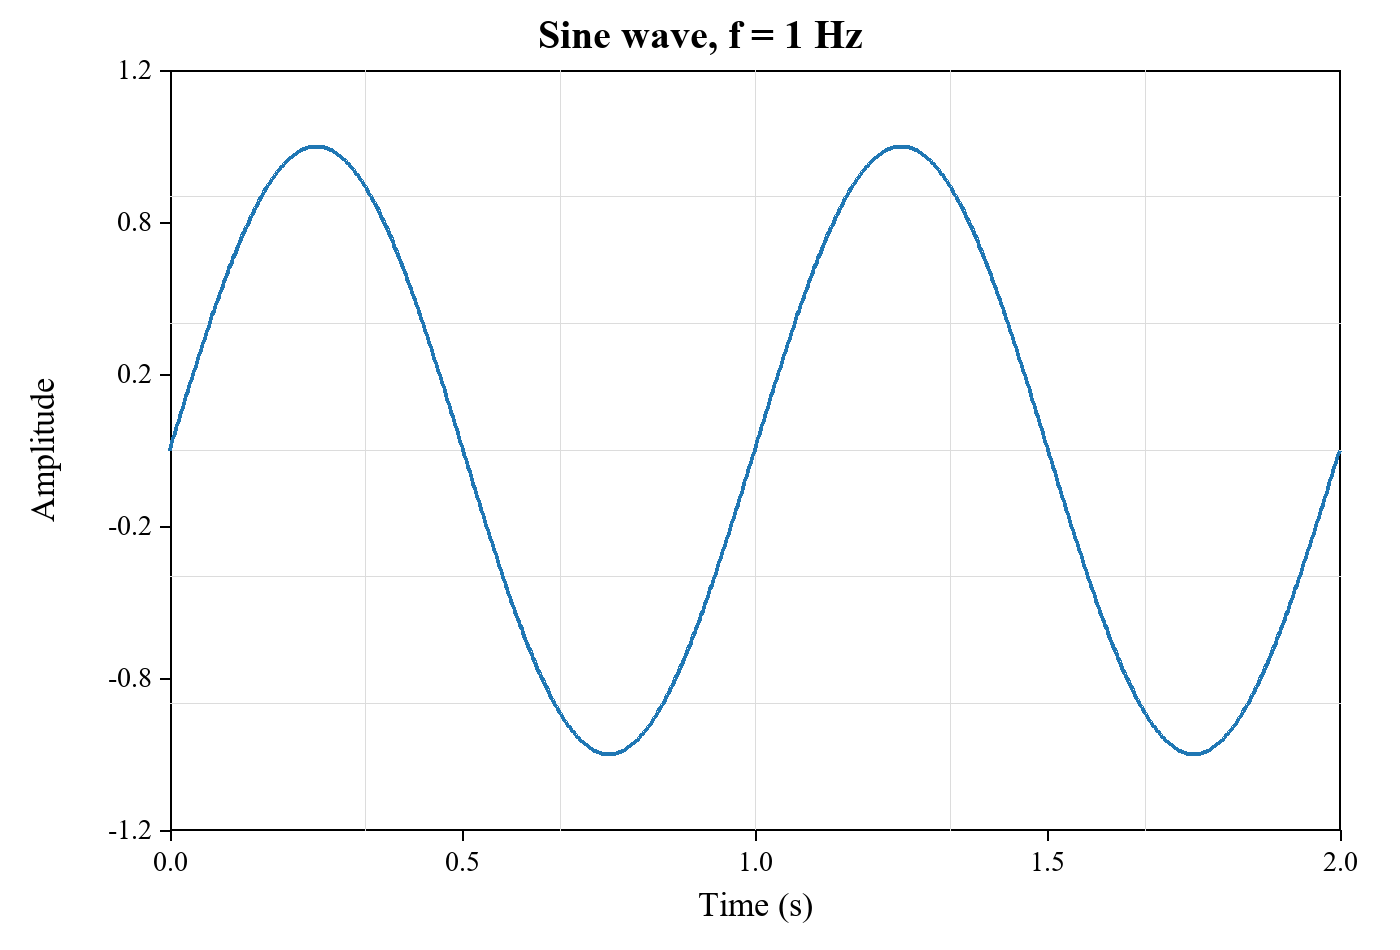
\includegraphics[width=\linewidth]{figure/fig_sine.png}
  \caption{远场平面波近似}\label{fig:sine}
\end{subfigure}
\hfill
\begin{subfigure}[b]{0.47\linewidth}
  \centering
  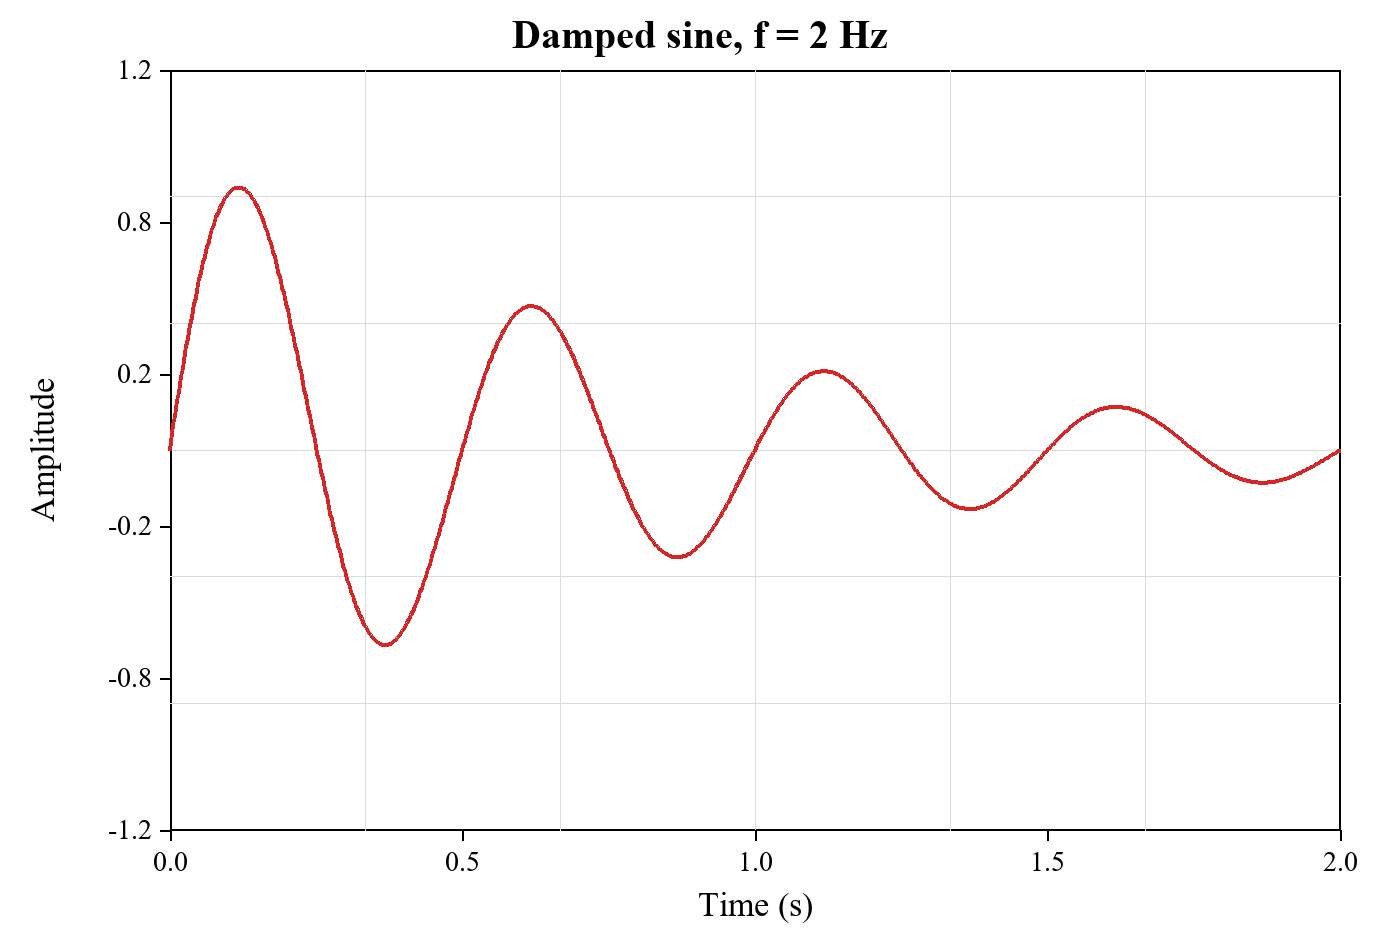
\includegraphics[width=\linewidth]{figure/fig_damped.png}
  \caption{近场球面波聚焦}\label{fig:damped}
\end{subfigure}
\caption{两种信道模型下的归一化波束图样对比}\label{fig:wave}
\end{figure}

% EPS 图片示例：把 .eps 文件放入 figure/ 后取消下面注释即可使用（需要 Ghostscript）：
% \begin{figure}[htbp]
%   \centering
%   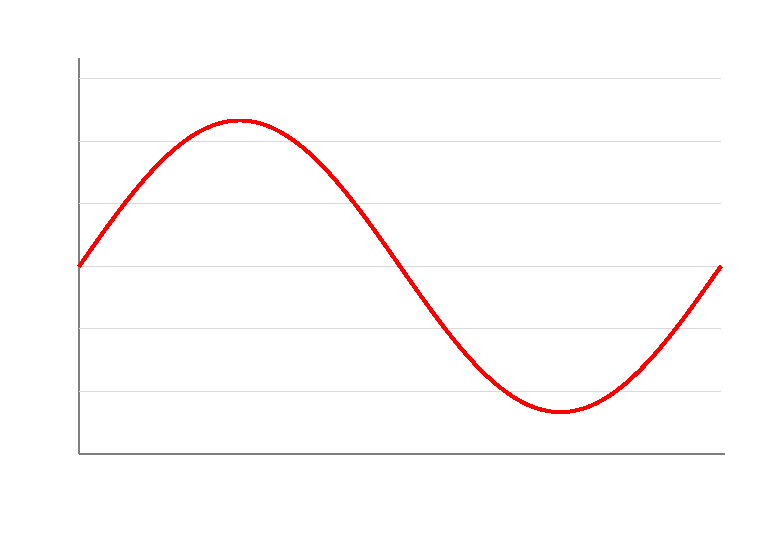
\includegraphics[width=0.7\linewidth]{figure/fig_eps_demo.eps}
%   \caption{EPS 矢量图示例}\label{fig:epsdemo}
% \end{figure}

表\ref{tab:diagbox}给出了不同场景与算法组合下的归一化吞吐量。以穷举法为基准（归一化为1.00），本文算法在视距场景下达到0.98，明显优于迫零预编码的0.82；在非视距场景下，本文算法的优势进一步扩大。这表明交替优化能够有效缓解用户间干扰。

\begin{table}[htbp]
\centering
\caption{不同场景下的归一化吞吐量}\label{tab:diagbox}
\zihao{5}
\begin{tabular}{c|ccc}
\hline
\diagbox[width=8em]{场景}{算法} & 穷举法 & 交替优化 & 迫零预编码 \\
\hline
视距（LoS）    & 1.00 & 0.98 & 0.82 \\
非视距（NLoS） & 1.00 & 0.95 & 0.71 \\
混合场景       & 1.00 & 0.97 & 0.78 \\
\hline
\end{tabular}
\end{table}

综合图\ref{fig:wave}与表\ref{tab:diagbox}可知，所提算法在保证用户公平性的前提下显著提升了系统吞吐量，且复杂度低于穷举法，验证了第\ref{sec:algo}节的理论分析。

\section{结论}\label{sec:concl}

本文研究了6G近场NOMA系统的联合波束成形与功率分配问题，建立了兼顾公平性与吞吐量的优化模型，提出了基于交替优化的迭代算法并证明了其收敛性。仿真结果表明，与迫零预编码和等功率分配方案相比，所提算法的系统吞吐量分别提升约18.6\%和25.3\%。后续工作将考虑信道估计误差与硬件损伤对算法性能的影响。

% --------------------------- 参考文献 ----------------------------------------
% GB/T 7714 顺序编码制：使用 bibtex + gbt7714-numerical.bst
% 注意：gbt7714 已自动加载 natbib，故不再加载 cite 与 citesort（见 README）
\bibliographystyle{gbt7714-numerical}
\bibliography{mybib}

\end{document}
